\begin{figure}[t]
\centering
\mpage{0.3}{
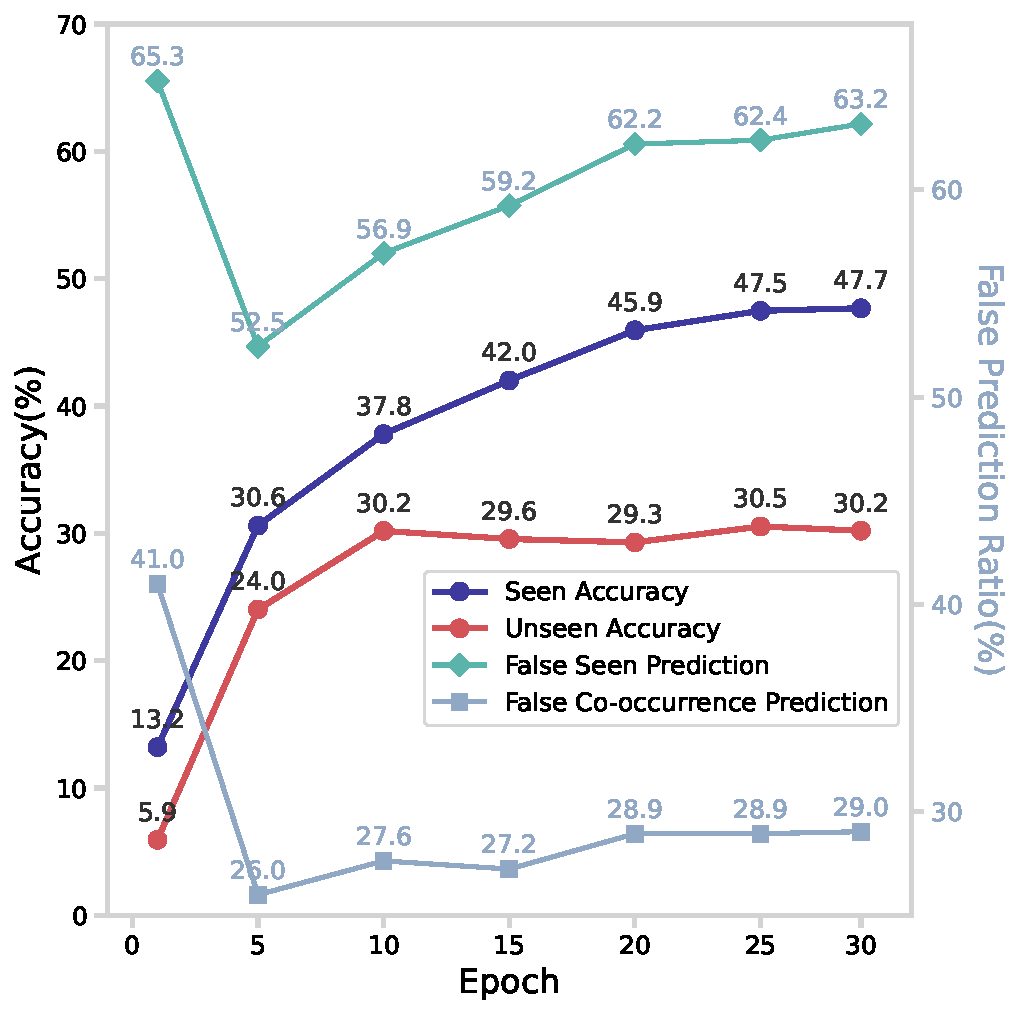
\includegraphics[width=\linewidth]{figure/src/diagnosis/diagnosis_learning_curve_clip_re_FCP.pdf}
}
\mpage{0.3}{
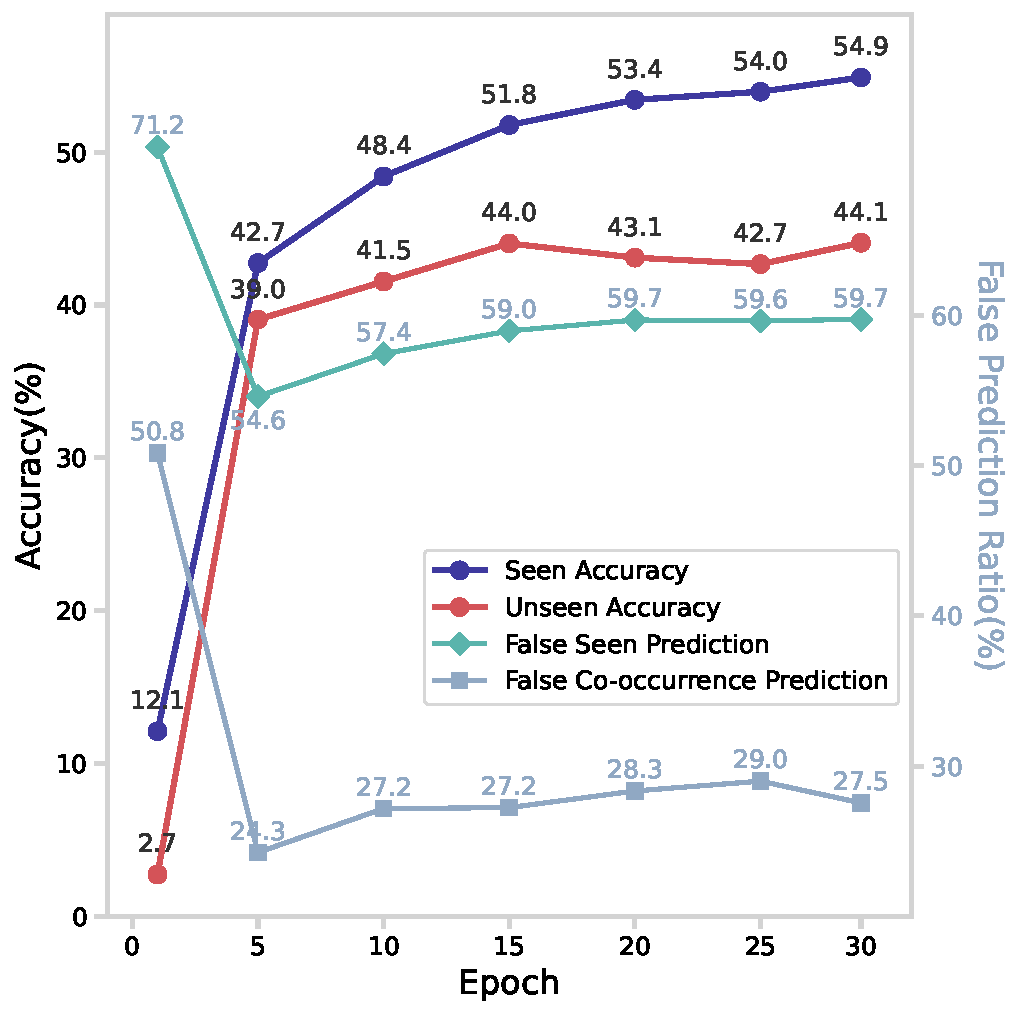
\includegraphics[width=\linewidth]{figure/src/diagnosis/diagnosis_learning_curve_iv2_re_FCP.pdf}
}
\mpage{0.26}{
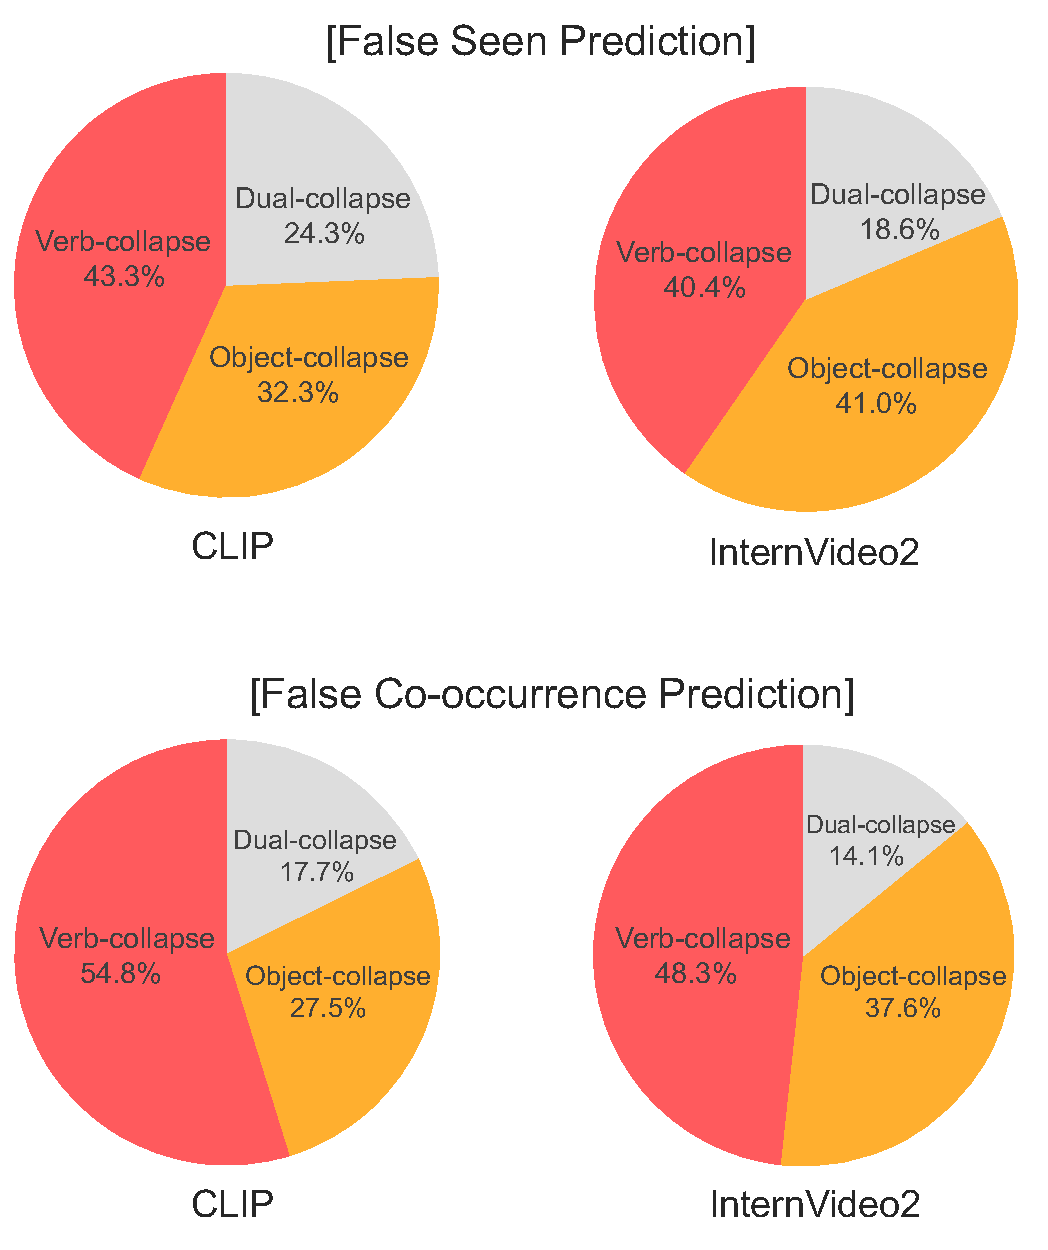
\includegraphics[width=\linewidth]{figure/src/diagnosis/pie_charts.pdf}
}
\\
\vspace{-1em}
\mpage{0.3}{
\scriptsize{(a) CLIP}
}
\mpage{0.3}{
\scriptsize{(b) InternVideo2}
}
\mpage{0.26}{
\scriptsize{(c) FSP/FCP breakdown}
}
\\
\figcapmargin
\vspace{-.8em}
\figcaption{Shortcut reliance correlates with poor unseen generalization}{
We show learning curves of C2C~\cite{li2024c2c} on Sth-com with CLIP~\cite{radford2021clip} and InternVideo2~\cite{wang2024iv2}.
(a) With CLIP, the seen–unseen accuracy gap grows together with FSP/FCP, indicating strong overfitting to seen compositions.
(b) Even with the video-pretrained InternVideo2 backbone, the model still shows a notable seen–unseen gap and high FSP.
(c) FSP/FCP breakdown at the final epoch: CLIP is dominated by verb-collapse due to object-driven shortcuts, while InternVideo2 exhibits milder but persistent shortcut behavior.
Best viewed with zoom and color.
}

\label{fig:diagnosis_baseline}
\end{figure}



